%%%%%%%%%%%%%%%%%%%%%%%%%
% Dokumentinformationen %
%%%%%%%%%%%%%%%%%%%%%%%%%
\newcommand{\titleinfo}{Wechsel- \& Drehstromtechnik - Formelsammlung}
\newcommand{\authorinfo}{Braun \& Co, J.Rast}
\newcommand{\versioninfo}{$Revision: 1 $ - powered by \LaTeX}

%%%%%%%%%%%%%%%%%%%%%%%%%%%%%%%%%%%%%%%%%%%%%
% Standard projektübergreifender Header für
% - Makros 
% - Farben
% - Mathematische Operatoren
%
% DORT NUR ERGÄNZEN, NICHTS LÖSCHEN
%%%%%%%%%%%%%%%%%%%%%%%%%%%%%%%%%%%%%%%%%%%%%
% Genereller Header
\documentclass[10pt,twoside,a4paper,fleqn]{article}
\usepackage[utf8]{inputenc}
\usepackage[left=1cm,right=1cm,top=1cm,bottom=1cm,includeheadfoot]{geometry}
\usepackage[ngerman]{babel,varioref}

% Pakete
\usepackage{amssymb,amsmath,fancybox,graphicx,color,lastpage,wrapfig,fancyhdr,hyperref,verbatim,booktabs,multirow}

%%%%%%%%%%%%%%%%%%%%
% Generelle Makros %
%%%%%%%%%%%%%%%%%%%%
\newcommand{\formelbuch}[1]{$_{\textcolor{red}{\mbox{\small{S#1}}}}$}
\newcommand{\verweis}[2]{\small{(siehe auch \ref{#1}, #2 (S. \pageref{#1}))}}
\newcommand{\subsubadd}[1]{\textcolor{black}{\mbox{#1}}}


\newcommand{\skriptsection}[2]{\section{#1 {\tiny Skript S. #2}}}
\newcommand{\skriptsubsection}[2]{\subsection{#1 {\tiny Skript S. #2}}}
\newcommand{\skriptsubsubsection}[2]{\subsubsection{#1 {\tiny Skript S. #2}}}

%%%%%%%%%%
% Farben %
%%%%%%%%%%
\definecolor{black}{rgb}{0,0,0}
\definecolor{red}{rgb}{1,0,0}
\definecolor{white}{rgb}{1,1,1}
\definecolor{grey}{rgb}{0.8,0.8,0.8}

%%%%%%%%%%%%%%%%%%%%%%%%%%%%
% Mathematische Operatoren %
%%%%%%%%%%%%%%%%%%%%%%%%%%%%
\DeclareMathOperator{\sinc}{sinc}
\DeclareMathOperator{\Real}{Re}
\DeclareMathOperator{\Imag}{Im}



% Fouriertransformationen
\unitlength1cm
\newcommand{\FT}
{
\begin{picture}(1,0.5)
\put(0.2,0.1){\circle{0.14}}\put(0.27,0.1){\line(1,0){0.5}}\put(0.77,0.1){\circle*{0.14}}
\end{picture}
}


\newcommand{\IFT}
{
\begin{picture}(1,0.5)
\put(0.2,0.1){\circle*{0.14}}\put(0.27,0.1){\line(1,0){0.45}}\put(0.77,0.1){\circle{0.14}}
\end{picture}
}



%%%%%%%%%%%%%%%%%%%%%%%%%%%%
% Allgemeine Einstellungen %
%%%%%%%%%%%%%%%%%%%%%%%%%%%%
%pdf info
\hypersetup{pdfauthor={\authorinfo},pdftitle={\titleinfo},colorlinks=false}
\author{\authorinfo}
\title{\titleinfo}

%Kopf- und Fusszeile
\pagestyle{fancy}
\fancyhf{}
%Linien oben und unten
\renewcommand{\headrulewidth}{0.5pt} 
\renewcommand{\footrulewidth}{0.5pt}

\fancyhead[L]{\titleinfo{ }\tiny{(\versioninfo)}}
%Kopfzeile rechts bzw. aussen
\fancyhead[R]{Seite \thepage { }von \pageref{LastPage}}
%Fusszeile links bzw. innen
\fancyfoot[L]{\footnotesize{\authorinfo}}
%Fusszeile rechts bzw. ausen
\fancyfoot[R]{\footnotesize{\today}}

% Einrücken verhindern versuchen
\setlength{\parindent}{0pt}



% Möglichst keine Ergänzungen hier, sondern in header.tex
\begin{document}

%%%%%%%%%%%%%%%%%%%%%%%%%%%%%%%%%%%%%%%%%%%%%%%%%%%%%%%%%%%%%%%%%%%%%%%%%%%%%%%%%%%%%%%%%%%%%%%%
\section{Wechselstromtechnik}
	\subsection{Periodisch zeitabhängige Grössen}
 %		\subsubsection{Periodische Schwingungen}
 %			\begin{tabular}{p{6cm}p{4.5cm}p{7.5cm}}
 %				Frequenz &
 %           		\fbox{$f = \frac{1}{T} = \frac{2 \pi}{\omega}$} &
 %            		$[f] = s^{-1}$ \\ \\
 %				Schwingungsbreite &
 %					\fbox{$i_{pp} = i_{max} - i_{min}$} \\ \\
 %				Scheitelwert &
 %					\fbox{$\hat{i} = |i_{max}| \quad\text{für}\quad{|i_{max}|}\geq{|i_{min}|} \quad \text{oder} \quad \hat{i} = |i_{min}|\quad\text{für}\quad |i_{max}| < |i_{min}|$}
 %			\end{tabular}
		\subsubsection{Gleichrichterschaltungen}
			\begin{tabular}{p{4cm}p{4cm}p{9cm}}
            	\begin{minipage}{4cm}
            		\textbf{Einweggleichrichtung} \\
            		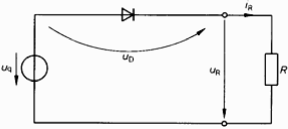
\includegraphics[height=1.2cm]{./bilder/EinwegGleichrichtung.png}
            	\end{minipage} &
            		\begin{minipage}{4cm}
                    	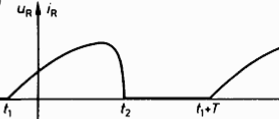
\includegraphics[width=4cm]{./bilder/AusgangsspannungStromEinwegGleichrichtung.png}
                    \end{minipage} &
					\begin{minipage}{8cm}
                    	Fliesst nur ein Strom in Durchlassrichtung der Diode. \\
                    	Summe der Oberwellen $i_0=0.2176A$ \\
                    	$t_1 < t < t_2$ $\Rightarrow$ $u_R = u_q$ ; $i_R = u_q/R$ ; $u_D = 0$ \\
                    	$t_2 < t < (t_1+T)$ $\Rightarrow$ $u_R = 0$ ; $i_R = 0$ ; $u_D = u_q$
                    \end{minipage} \\
				\begin{minipage}{4cm}
                	\textbf{Zweiweggleichrichtung} \\
                	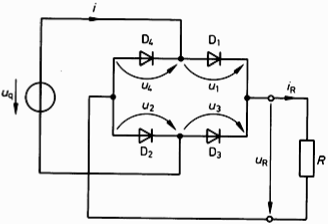
\includegraphics[height=1.5cm]{./bilder/BrueckenGleichrichtung.png}
                \end{minipage} &
					\begin{minipage}{4cm}
                    	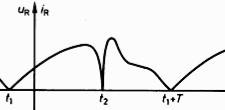
\includegraphics[width=4cm]{./bilder/AusgangsspannungBrueckenGleichrichtung.png}
                    \end{minipage} &
					\begin{minipage}{9cm}
                    	Ausgangsspannung ist Betrag der Eingangsspannung. \\
                    	$t_1 < t < t_2$ $\Rightarrow$ $D_1,D_2$ leiten ; $D_3,D_4$ sperren \\
                    	$t_2 < t < (t_1+T)$ $\Rightarrow$ $D_1,D_2$ sperren ; $D_3,D_4$ leiten \\
                    	$u_R = |u_q|$ ; $i_R = u_R/R = |i|$
                    \end{minipage}
            \end{tabular}

		\subsubsection{Mittelwerte periodischer Grössen}
			\begin{tabular}{p{5.5cm}p{5cm}p{7.5cm}}
			Arithmetischer Mittelwert, Gleichwert, Linearer MW &
	$X_0 = \overline{X} = X_m = \frac {1} {T} \int\limits_{t_0}^{t_0+T} x(t)dt$ &
	\begin{minipage}{7.5cm}
    		Ist die Fl\"ache unter der Zeitfunktion über eine Periode.
    \end{minipage} \\
Quadratischer MW, Leistung &
	$X^2 = \frac {1} {T} \int\limits_{t_0}^{t_0+T} x^2(t)dt$ & 
	$X^n = \frac {1} {T} \int\limits_{t_0}^{t_0+T} x^n(t)dt$ (MW $n$. Ordnung) \\
Effektivwert &
	$X = X_{\text{eff}}= \sqrt{X^2} = \sqrt{\frac{1}{T} \int\limits ^{t_0+T} _{t_0}{x^2(t)dt}}$
	& \\ Gleichrichtwert &
	$X_{|m|} = \bar{|X|} = \frac{1}{T} \int\limits_{t_0}^{t_0+T}{|x(t)| dt}$ &
	\begin{minipage}{7.5cm}
    	Arithm. Mittelwert der Zweiweggleichrichterschaltung
    \end{minipage} \\

				Energie der Periode $T$ &
					\fbox{$W_T = \int\limits_{t_0}^{t_0+T}{P(t) dt}$} &
					\begin{minipage}{7.5cm}
                    	ist die Energie positiv, nimmt der Zweipol Energie auf
                    \end{minipage} \\
				Wirkleistung &
					\fbox{$P = \frac{1}{T} \int\limits_{t_0}^{t_0+T}{P(t) dt}$} \\ \\
			\end{tabular}
 
			\begin{tabular}{p{5.5cm}p{5cm}p{7.5cm}}
				\textbf{Verhältniszahlen}
				&	Scheitelfaktor $k_s$ (crest factor): &
						$k_s = \frac{\text{Scheitelwert}}{\text{Effektivwert}} = \frac{\hat{u}}{U}$ \\ \\
				&	Formfaktor F (form factor): &
						$F = \frac{\text{Effektivwert}}{\text{Gleichrichtwert}} = \frac{U}{|\bar{u}|}$ \\ \\
				&	Schwingungsgehalt: &
						$s = \frac{\text{Effektivwert des Wechselsignals}}{\text{Effektivwert der Mischgrösse}}$ \\ \\
				&	Effektive Welligkeit: &
						$\frac{\text{Effektivwert des Wechselsignals}}{\text{Gleichwert der Mischgrösse}}$ \\ \\
				&	Riffelfaktor: &
						$\frac{\text{Scheitelwert des Wechselsignals}}{\text{Gleichwert der Mischgrösse}}$ \\ \\
			\end{tabular}

			\begin{tabular}{p{5.5cm}p{5cm}p{7.5cm}}
				\textbf{Simpsonsche Regel}
				&	Gleichwert: &
						$\bar{i} = \frac{h}{3T} \sum m \cdot i$ \\ 
				\textit{(Berechnungsmethode anhand}		\\
				
				\textit{eines Graphen) }
				 &	Gleichrichtwert: &
						$|\bar{i}| = \frac{h}{3T} \sum m \cdot |i|$ \\ \\
						
				 &	Effektivwert: &
						$I_{eff} = \sqrt{\frac{h}{3T} \sum m \cdot i^2}$ \\ \\
				\begin{minipage}{4.5cm}
					\begin{tabular}{| c | c | c | c | c | c | c | c |}
						\hline
			 				$n$ & $t$ &$i$ & $i^2$ & $m$ & $m \cdot i$ & $m \cdot i^2$ \\
			 			\hline
				 			1 & & & & 1 & & \\
				 		\hline
				 			2 & & & & 2 & & \\
				 		\hline
				 			3 & & & & 4 & & \\
				 		\hline
				 			4 & & & & 2 & & \\
				 		\hline
				 			5 & & & & 1 & & \\
				 		\hline
			 		\end{tabular}
				\end{minipage} &
				\begin{minipage}{12.5cm}
                	Wähle im Graph der Aufgabenstellung, das den Strom i(t) darstellt, innerhalb
					der Periode $T$ eine ungerade Anzahl von $\boldsymbol{n}$ \textbf{Stützstellen} in konstanten
					\textbf{Abständen }$\boldsymbol{h}=\frac{T}{n-1}$ (z.B $T=20ms, n=11$ mit $h=2 ms$). Lese an
					diesen Stellen jeweils den Augenblickswert des Stromes ab und tragen ihn in eine Tabelle ein (s.l). Berechne anschliessend für jede 
					Stützstelle den Wert von $i^2$ und den Summanden $m \cdot i^2$. Der \textbf{Faktor}
					$\boldsymbol{m}$ wird wie folgt gebildet: Für ungerade n ist m=4; bei der ersten und bei der
					letzten Stützstelle ist m=1, bei den übrigen ist m=2.
                \end{minipage}
			\end{tabular}
	\subsection{Sinusförmige Schwingungen von Spannung und Strom}
% 		\subsubsection{Erzeugung sinusförmiger Schwingungen}
% 			\begin{minipage}[t]{6cm}
%             	\textbf{Bewegte Leiter im \\ homogenen Magnetfeld}
%             \end{minipage}
% 			\begin{minipage}[lt]{4.5cm}
%             	$U = B \cdot l \cdot v$ \\
%             	$v_q = v \cdot cos\beta$ $\quad (v_p = v \cdot sin\beta)$ \\
%             	$U = \hat{U} \cdot sin\alpha$
%             \end{minipage}
% 			\begin{minipage}{3.5cm}
%             	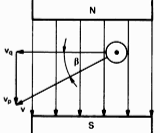
\includegraphics[width=3.5cm]{./bilder/BewegteLeiter.png}
%             \end{minipage}
% 			\begin{minipage}{3.5cm}
%             	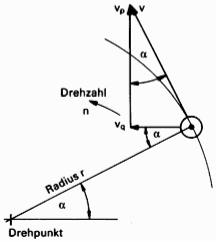
\includegraphics[width=3.5cm]{./bilder/KreisfoermigeBewegung.png}
%             \end{minipage}
% 		\subsubsection{Beschreibung sinusförmiger Spannungen und Ströme}
% 			\begin{tabular}{p{6cm}p{4.5cm}p{7.5cm}}
%             	\textbf{Kreisfrequenz} &
%             		\fbox{$\omega = \frac{2 \pi}{T} = 2 \pi f$} &
%             		$[\omega] = s^{-1}$ \\ \\
%             	\textbf{Effektivwert für sinusförmige Grössen} &
%             		\fbox{$U = \frac{\hat{u}}{\sqrt{2}} \quad I = \frac{\hat{i}}{\sqrt{2}}$}
%             \end{tabular}
		\subsubsection{Komplexe Zeiger}
			\begin{minipage}[t]{6cm}
            	\textbf{Prinzip der Zeigertechnik}
            \end{minipage}
			\begin{minipage}{6cm}
            	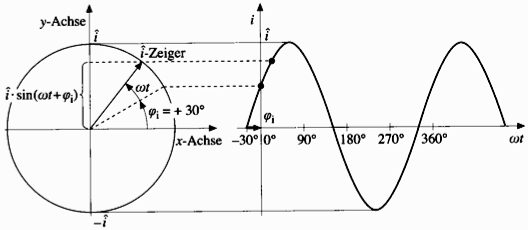
\includegraphics[width=6cm]{./bilder/RotierenderScheitelwertzeiger.png}
            \end{minipage}
			\begin{minipage}{3.5cm}
            	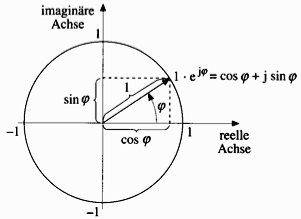
\includegraphics[width=3.5cm]{./bilder/EulerscheRelation.png}
            \end{minipage} \\
			\begin{tabular}{p{5cm}p{4.5cm}p{8.5cm}}
            	Komplexer Effektivwert &
            		$\underline{U} = \frac{\underline{\hat{u}}}{\sqrt{2}}$ &
            		$\underline{U}$ = Kompl. Effektivwert, $\underline{\hat{u}}$ = Kompl. Scheitelwert \\
				Exponentialform &
					$\underline{\hat{u}} = \hat{u} \cdot e^{j\varphi_u} \quad \underline{U} = U \cdot e^{j\varphi_U}$ \\
				Algebraische Form &
					$\underline{\hat{u}} = \hat{u} (\cos(\varphi_u)+j\sin(\varphi_u))$ &
					$\Real(\underline{\hat{u}}) = \hat{u} \cdot \cos(\varphi_u)$ \quad $\Imag(\underline{\hat{u}}) = \hat{u} \cdot \sin(\varphi_u)$ \\
				&	$\underline{U} = U (\cos(\varphi_U)+j\sin(\varphi_U))$ &
					$\Real(\underline{U}) = U \cdot \cos(\varphi_U)$ \quad $\Imag(\underline{U}) = U \cdot \sin(\varphi_U)$ \\
				Umrechnung &
					$|\hat{u}| = \sqrt{\Real(\underline{\hat{u}})^2 + \Imag(\underline{\hat{u}})^2}$ \quad $\varphi_u = \arctan\left(\dfrac{\Imag(\underline{\hat{u}})}{\Real(\underline{\hat{u}})}\right)$ \\
				&	$|U| = \sqrt{\Real(\underline{U})^2 + \Imag(\underline{U})^2}$ \quad $\varphi_U = \arctan\left(\dfrac{\Imag(\underline{U})}{\Real(\underline{U})}\right)$ \\
				Komplexe Drehzeiger &
					$\underline{u}(t) = \underline{\hat{u}} \cdot e^{j\omega t} = \hat{u} \cdot e^{j\varphi_u} \cdot e^{j\omega t} = \hat{u} \cdot e^{j(\omega t + \varphi_u})$ \\
				Phasenwinkel &
					$\varphi = \varphi_u - \varphi_i$ &
					Phasenwinkel positiv $\rightarrow$ Spannung eilt Strom voraus (im Gegenuhrzeigersinn) \\
			\end{tabular}
		\subsubsection{Komponenten linearer Wechselstromnetzwerke}% \formelbuch{125}}
			\begin{tabular}{llll}
			$\underline{Z} = R +j X$: 
				& Komplexer Widerstand (Impedanz); 
				& $R$: Wirkwiderstand (Resistanz); 
				& $X$: Blindwiderstand (Reaktanz)\\
			$\underline{Y} = G + j B$: 
				& Komplexer Leitwert (Admittanz); 
				& $G$: Wirkleitwert (Konduktanz); 
				& $B$: Blindleitwert (Suszeptanz)
	      	\end{tabular} \\ \\
			\begin{tabular}{p{2cm}p{12cm}p{5cm}}
				\textbf{Widerstand} &
					$ \boxed{\underline{Z_R} = R} \quad \boxed{\underline{Y} = G =
					\frac{1}{R}}$ &
						\begin{minipage}{8cm}
	                    	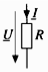
\includegraphics[height=1cm]{./bilder/Wirkwiderstand.png}
	                    	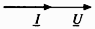
\includegraphics[width=1cm]{./bilder/WirkwiderstandZeiger.png}
	                    \end{minipage} \\ \\
				\textbf{Induktivität} &
					$ \boxed{\underline{Z_L} = j \omega L = j X_L} \quad
					\boxed{\underline{Y_L} = - \frac{j}{\omega L} = j B_L} \quad
					\boxed{W_L=\frac12 L I_L^2}$ &
						\begin{minipage}{8cm}
		                    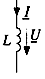
\includegraphics[height=1cm]{./bilder/Spule.png}
		                    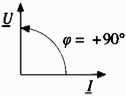
\includegraphics[width=1cm]{./bilder/SpuleZeiger.png}
		                \end{minipage} \\ \\
				\textbf{Kondensator} &
					$ \boxed{\underline{Z_C} = \frac{1}{j \omega C} = - \frac{j}{\omega C} = j
					X_C \quad (X_C < 0)} \quad \boxed{\underline{Y_C} = j \omega C = j B_C} \quad
					\boxed{W_C=\frac12 C U_C^2}$ &
						\begin{minipage}{8cm}
		                    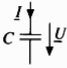
\includegraphics[height=0.8cm]{./bilder/Kondensator.png}
		                    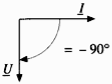
\includegraphics[width=1cm]{./bilder/KondensatorZeiger.png}
		                \end{minipage} \\ \\
			\end{tabular}
		\subsubsection{Berechnung linearer Wechselstromnetzwerke}
		\subsubsection{Leistung im Wechselstromnetzwerk}% \formelbuch{162}}
				\begin{tabular}{p{7cm}p{4.5cm}p{7cm}}
					Komplexe Leistung &
						\fbox{$ \underline{S} = \underline{U} \cdot \underline{I}^\ast = U\cdot I \cdot e^{j(\varphi_u-\varphi_i)}$ }  &
						Konjugiert Komplexer Strom! \\
					Wirkleistung &
						\fbox{$ P = \Real(\underline{S}) = U I \cos(\varphi) $ } \\
					Blindleistung &
						\fbox{$ Q = \Imag(\underline{S}) = U I \sin(\varphi) $ } &
						Kapazitiv: $Q < 0$; induktiv: $Q > 0$ \\
					Scheinleistung &
						\fbox{$ S = | \underline{S} | = U I = \frac{U^2}{R} = I^2 R$ } \\
					Leistungsfaktor &
						\fbox{$\lambda = \frac{P}{S} = \frac{P}{UI} = \cos \varphi$} \\
				\end{tabular}
		\subsubsection{Blindleistungskompensation (mit Kondensator)}
		\renewcommand{\arraystretch}{1.5}
\begin{tabular}{p{7cm}p{4.5cm}p{5cm}}
	Kompensation mit C &
    	\begin{minipage}{4cm}
        	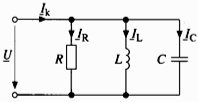
\includegraphics[width=3.5cm]{bilder/Parallelkompensation.png}
        \end{minipage} & 
		Der Kondensator wird parallel dazu geschalten \\ \\
	Zeigerdiagramme Kompensation &
		\begin{minipage}{4.5cm}
        	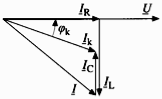
\includegraphics[width=3.5cm]{bilder/Blindstromkompensation.png}
        \end{minipage} &
		\begin{minipage}{4.5cm}
        	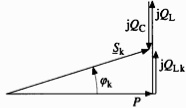
\includegraphics[width=3.5cm]{bilder/Blindleistungskompensation.png}
        \end{minipage} \\ \\
	Neue (kompensierte) Blindleistung &
		$Q_{Lk} = P \cdot \tan{\varphi_k}$ \\
	Blindleistung des Kondensators & 
		\multicolumn{2}{l}{$Q_C = Q_{Lk} - Q_L =  P\cdot (\tan{\varphi_k}-\tan{\varphi}) $} \\
	Kapazität des Kondensators &
		$C = - \frac{Q_C}{\omega U^2}$ \\	
	\end{tabular}
\renewcommand{\arraystretch}{1}
		
		\subsubsection{Leistungsumsatz bei nichtsinusförmigen periodischen Grössen}
		\begin{minipage}[c]{7.5cm}
			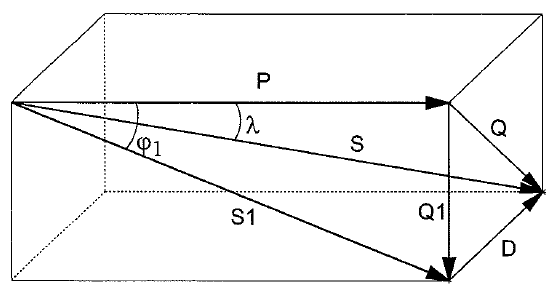
\includegraphics[height=4cm]{../WS_DST/bilder/ZeigerdiagrammNichtSinus.png}     
    	\end{minipage}
		\begin{minipage}[c]{10.5cm}   
    		\noindent
    		\renewcommand{\arraystretch}{2.5}
    		\begin{tabular}{p{1.8cm} p{5.6cm}}
        		Unterwelle: 
        		& $X_{U} = \overline{X} = \dfrac{\hat{X}}{\sqrt{2}} a_0 \qquad $  \\
	     		Grundwelle: 
	     		& $X_{G} = \dfrac{\hat{X}}{\sqrt{2}} \sqrt{a_1^2 + b_1^2} \qquad  $   \\
	     		Oberwellen: 
	     		& $X_{O} = \dfrac{\hat{X}}{\sqrt{2}}
	     		\sqrt{\sum\limits_{k=2}^{\infty}a_k^2 +\sum\limits_{k=2}^{\infty}b_k^2}
	     		\qquad $  \\ \multicolumn{2}{l}{Effektivwerte: $X_{RMS} = \sqrt{X_G^2 + X_O^2} \qquad X_{TRMS} =
	     		\sqrt{X_U^2 + X_{RMS}^2}$ } \\
		\multicolumn{2}{l}{ges. Blindleistung: $Q = \sqrt{Q_G^2 + Q_U^2 + U^2
		\sum\limits_{k=2}^{\infty}I_k^2} = \sqrt{U^2 \sum\limits_{k=0}^{\infty}I_k^2}$} \\ 
		\multicolumn{2}{l}{Verzerrungsblindleistung: $D = U
		\cdot \sqrt{I_0^2 + \sum\limits_{k=2}^{\infty}I_k^2}$} \\
		\multicolumn{2}{l}{ges. Scheinleistung: $S = \sqrt{P^2 + Q^2 + D^2} = U \cdot I_{TRMS}$} \\
		 \end{tabular} \\
		 \renewcommand{\arraystretch}{1}
     	\end{minipage}    		\\ \\
     	Die Verzerrungsblindleistung wird von den Oberwellen und ev. von der Unterwelle (je
     	nach Phasenverschiebung) verursacht und ist mit Kondensatoren \textbf{nicht} zu kompensieren -
     	Aktive Filter wären nötig.
		\\		
		
	\begin{minipage}[c]{8cm} 
	   \textbf{Beispiel anhand eines Einweggleichrichters:}	  	\\
	   (mit ohmscher Last R) 
	\end{minipage}   
	\begin{minipage}[c]{10cm} 	
	   $ \qquad i(t) = \underbrace{\frac{A}{\pi}}_{Unterwelle} + \underbrace{\frac{A}{2}
	   \sin(t)}_{Grundwelle} - \underbrace{\frac{2A}{\pi} \sum\limits_{k=1}^n \frac{1}{(2k-1)(2k+1)} \cos(2kt)}_{Oberwellen} $
	\end{minipage}   
		
	\begin{minipage}[c]{10cm}  
		\begin{tabular}{| l | l |}
    		\hline 
      		\textbf{Bezeichnung}
      		%& \textbf{Näherungsformel}
      		& \textbf{Formel} \\
      		\hline
      		Scheitelwert 
      		%& %& $\hat{I} = 0.7071 \cdot A $
      		& $\hat{I} = \hat{I}_d = \frac{\hat{U}_d}{R} $ \\
      		Unterwelle (Mittelwert)
      		%& $I_U = 0.22508 \cdot A $
      		& $I_U = \bar{I}_d = \frac{\hat{I}}{\pi}$ \\
      		Grundwelle
      		%& $I_G = 0.25 \cdot A$ 
      		& $I_G = \frac{\hat{I}}{2 \cdot \sqrt{2}}$ \\
      		Oberwelle
      		%& $I_O = 0.10881 \cdot A$ 
      		& $I_O = \frac{\hat{I}}{\sqrt{2}} \cdot 0.21762$ \\
      		%Effektivwert (RMS)
      		%& $I_{RMS} = 0.27265 \cdot A$
      		%& $I_{RMS} = \sqrt{I_G^2 + I_O^2}$ \\
      		Laststrom
      		%& $I_{TRMS} = 0.35355 \cdot A$
      		& $I_{d} =\frac{\hat{U}_s}{2 R}$ \\
      		Primärstrom
      		& $I_1 \approx I_U \cdot \frac{1.21}{"u}$ \\
      		Bauleistung 
      		& $S_{TR} = \frac{S_{1Tr} + S_{2Tr}}{2}$ \\
      		\hline 
    	\end{tabular}
	\end{minipage}   
	\begin{minipage}[c]{8cm}  
			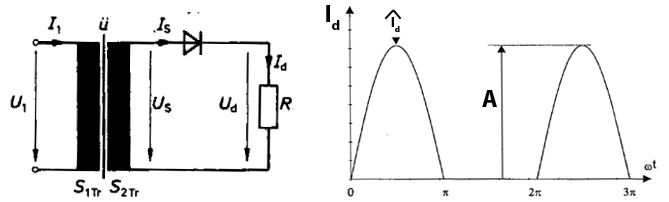
\includegraphics[width=8cm]{../WS_DST/bilder/EinwegGR.png}  \\			
	$S_{1Tr} < S_{2Tr}$ da der Trafo keine Gleichströme überträgt. Somit erscheint der Primärstrom
	als Sekundärstrom mit unterdrücktem Gleichstromanteil.			
	\end{minipage}

\newpage

	\begin{minipage}[c]{8cm} 
	   \textbf{Beispiel anhand eines Brückengleichrichters:}	  	\\
	   (mit ohmscher Last R)
	\end{minipage}   
	\begin{minipage}[c]{10cm} 	
	   $ \qquad i(t) = \underbrace{\frac{2A}{\pi}}_{Unterwelle} - \underbrace{\frac{4A}{\pi} \sum\limits_{k=1}^n \frac{1}{(2k-1)(2k+1)} \cos(2kt)}_{Oberwellen} $
	\end{minipage}\\
\begin{minipage}[c]{10cm}  
		\begin{tabular}{| l | l |}
    		\hline 
      		\textbf{Bezeichnung}
      		%& \textbf{Näherungsformel}
      		& \textbf{Formel} \\
      		\hline
      		Scheitelwert 
      		%& %& $\hat{I} = 0.7071 \cdot A $
      		& $\hat{I} = \hat{I}_d = \frac{\hat{U}_d}{R} $ \\
   %   		Fourien-Reihe
    %  		&$i(t)=A(\frac{2}{\pi}-\frac{4}{\pi}(\frac{\cos(2t)}{1\cdot
 %     		3}+\ldots+\frac{\cos(2nt)}{(2n-1) \cdot (2n+1)}))$\\
      		Unterwelle (Mittelwert)
      		%& $I_U = 0.22508 \cdot A $
      		& $I_U = \bar{I}_d = \frac{2 \hat{I}}{\pi}$ \\
      		Grundwelle
      		%& $I_G = 0.25 \cdot A$ 
      		& $I_G = 0$ \\
      		Oberwelle
      		%& $I_O = 0.10881 \cdot A$ 
      		& $I_O = \frac{\hat{I}}{\sqrt{2}} \cdot 0.43524$ \\
      		%Effektivwert (RMS)
      		%& $I_{RMS} = 0.27265 \cdot A$
      		%& $I_{RMS} = \sqrt{I_G^2 + I_O^2}$ \\ 
      		Laststrom
      		%& $I_{TRMS} = 0.35355 \cdot A$
      		& $I_{d eff} =  \frac{U_s}{R}= \frac{\hat{U}_d}{\sqrt{2}R}$ \\ 
      		Diodenstrom
      		& $I_{V} = \frac{\hat{U}}{2 R} = \frac{I_{d eff}}{\sqrt{2}}$ \\
      		Primärstrom
      		& $I_1 \approx I_U \cdot \frac{0.966}{"u}$ \\
      		Bauleistung 
      		& $S_{TR} = \frac{S_{1Tr} + S_{2Tr}}{2}$ \\
      		\hline
    	\end{tabular}
	\end{minipage}   
	\begin{minipage}[c]{8cm}  
			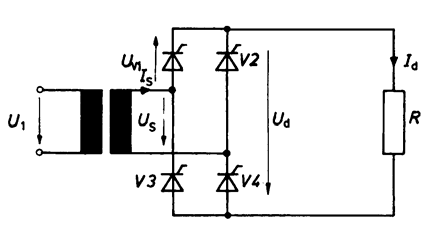
\includegraphics[width=7cm]{../WS_DST/bilder/brueckengleichrichter.png}  \\			
	$S_{1Tr} < S_{2Tr}$ da der Trafo keine Gleichströme überträgt. Somit erscheint der Primärstrom
	als Sekundärstrom mit unterdrücktem Gleichstromanteil.			
	\end{minipage}

\section{Transformator}
		
	\subsection{Trafomodelle}
%		\subsubsection{Grundstrucktur des Trafo}
%			\begin{tabular}{p{7cm}p{4.5cm}p{5cm}}
%	        	\textbf{} &
%	        		\begin{minipage}{4.5cm}
%		            	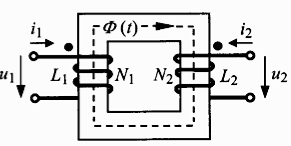
\includegraphics[width=3.5cm]{./bilder/GrundstruckturTrafo.png}
%		            \end{minipage} \\
%	        \end{tabular}
		\subsubsection{Der ideale Trafo}
			\begin{tabular}{p{7cm}p{4.5cm}p{5cm}}
				Übersetzungsverhältnis &
					$\text{ü} = \frac{|\underline{U}_1|}{|\underline{U}_2|} =
					\frac{|\underline{I}_2|}{|\underline{I}_1|} = \frac{N_1}{N_2}$ &
					\begin{minipage}{4.5cm}
						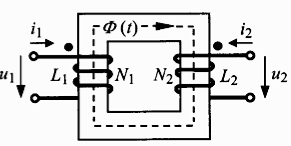
\includegraphics[width=3.5cm]{./bilder/GrundstruckturTrafo.png}
					\end{minipage} \\
				Leistungsbilanz &
					$\underline{S}_1 = \underline{S}_2$ &
					oder $\underline{U}_2 \cdot \underline{I}_2^* = \underline{U}_1 \cdot \underline{I}_1^*$ \\
				Scheinwiderstandsübersetztung &
					$\underline{Z}_{aU} = \frac{|\underline{U}_1|^2}{|\underline{U}_2|^2} \cdot \underline{Z}_a = \text{ü}^2 \cdot \underline{Z}_a$ &
					\begin{minipage}{4.5cm}
	            		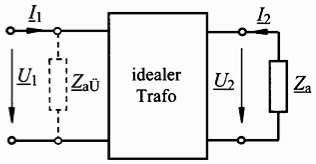
\includegraphics[width=3.5cm]{./bilder/IdealerTravoImpedanzwandler.png}
	            	\end{minipage}
			\end{tabular}
		\subsubsection{Verlustloser und Streuungsfreier Trafo}
			% trafo aus ET3 projekt
			\renewcommand{\arraystretch}{1.5}
\textbf{Induktionsgesetz}\\
		\begin{tabular}[c]{p{8.7cm}}
			$u_i= \mp \dot{\Phi} = \mp \frac{d}{dt} \int \vec{B} \cdot
			\vec{dA}\qquad $ \parbox{3cm}{\tiny{$- \Rightarrow B,u_i $
			Rechtsschraube\\ $+ \Rightarrow B,u_i $
			Linksschraube}}
			\\
			
			$u_i= \mp \dot{\Psi}\qquad$ , meist $\; u_i = \mp
			N\cdot\dot{\Phi}$		
		\end{tabular}
		\parbox{8cm}{Durchsetzt das sich \"andernde Magnetfeld einer stromdurchflossenen Spule
					eine zweite Spule, so wird auch in dieser eine Spannung
					(=Gegeninduktionsspannung) induziert.}	

\begin{multicols}{2}
 		\textbf{Gegeninduktion} ($M_{\textcolor{red}{X}\textcolor{green}{Y}}; \textcolor{red}{X}$: Wirkung,
 		$\textcolor{green}{Y}$: Ursache)\\
		\begin{tabular}{ll}
  		Gegeninduktivit\"at
  			& $M_{21} = \frac{\Psi_{m21}}{i_1}$ Meist $= \frac{N_2 \phi_{m21}}{i_1}$\\ 
  			(wenn $\mu$ = const.) & $M = k \cdot \sqrt{L_1 L_2} = M_{21} = M_{12} $  \\
  			Gegeninduktionsspannung
  			& $u_{21} = \dot{\Psi}_{21} = M_{21} \frac{di_1}{dt}$ \\
		\end{tabular}\\

  		\textbf{Transformatorgleichungen}\\
		$\boxed{u_1 = L_1 \dfrac{di_1}{dt} \textcolor{red}{+}\textcolor{green}{-}M_{12}
		\dfrac{di_2}{dt} = L_1 \dfrac{di_1}{dt} \textcolor{red}{-}\textcolor{green}{+}M_{12} \dfrac{di_b}{dt}}$ \\
		$\boxed{u_2 = L_2 \dfrac{di_2}{dt}\textcolor{red}{+}\textcolor{green}{-} M_{21}
		\dfrac{d i_1}{dt} = -L_2 \dfrac{di_b}{dt}
		\textcolor{red}{+}\textcolor{green}{-} M_{21} \dfrac{d i_1}{dt}}$\\
		Im Bildbereich:\\
		$\underline{U}_1 = j\omega\cdot L_1 \cdot \underline{I}_1 + j\omega\cdot M \cdot \underline{I}_2$\\
		$\underline{U}_2 = j\omega\cdot L_2 \cdot \underline{I}_2 + j\omega\cdot M \cdot \underline{I}_1$\\
  			
	  	\textbf{Idealer Trafo}\\ 
	  	$"u = \dfrac{u_1}{u_2} = \dfrac{N_1}{N_2} = \sqrt{\dfrac{L_1}{L_2}}$ $\qquad$ (im Leerlauf:
	  	$\dfrac{1}{"u} = k \sqrt{\dfrac{L_2}{L_1}}$)\\

  		\textbf{Verlustbehafteter Trafo}
  		\begin{list}{$\bullet$}{\setlength{\itemsep}{0cm} \setlength{\parsep}{0cm} \setlength{\topsep}{0cm}} 
          \item Prim\"arstrom im Leerlauf: $L_H$
          	(ideal $L_H \rightarrow \infty)$
          \item Hysterese- \& Wirbelstromverluste: $R_{Fe}$ \newline
          	(ideal: $R_{Fe}\rightarrow \infty$) 
          \item Kupferwiderst\"ande: $R_{Cu1}, R_{Cu2}$
          	(ideal: $R_{Cu}
          \rightarrow 0$)
          \item Streufluss (Kopplung): $L_{\sigma1}, L_{\sigma2}$
          	(ideal: $L_{\sigma} \rightarrow 0$)
        \end{list}

	\columnbreak
  		\begin{flushleft}
  		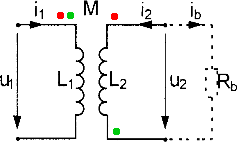
\includegraphics[width=4cm]{bilder/trafo-kopplung.png} \\
  		\small{\textcolor{red}{Gleichsinnig} / \textcolor{green}{Gegensinnig}} \\
  		\vspace{1cm}

	  	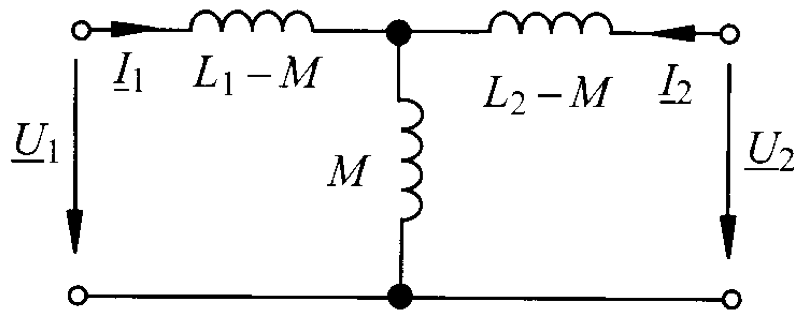
\includegraphics[width=5cm]{bilder/T_Ersatzschaltbild_VST.png}\\
		\end{flushleft}  	
	
\end{multicols}
\renewcommand{\arraystretch}{1} 	
		\subsubsection{Transformatoren-Hauptgleichung (gilt bei Leerlauf)}
			\begin{tabular}{p{7cm}p{4.5cm}p{5cm}}
      			\fbox{$| \hat{u}_{10} | = \hat{i}_0 \cdot X_{L1}$}
      			& 	\fbox{$\hat{u}_{10} = \hat{i}_0 \cdot \omega \cdot L_1$} \\
      		
				\fbox{$U_{20} = \frac{2\pi}{\sqrt{2}}N_2 f \hat{B}_1 A$}
				&
            	\fbox{$U_{10} = \frac{2\pi}{\sqrt{2}}N_1 f \hat{B}_1 A$} &
					wobei $\frac{2\pi}{\sqrt{2}} = 4.44$ und $\hat{B} \cdot A = \hat{\Phi}$ 
			\end{tabular}
	\subsection{Der reale (einphasige) Transformator}
		\subsubsection{Ersetzen der magnetischen Kopplung}
			\begin{tabular}{p{5.8cm}p{8cm}p{4.5cm}}
            	Spannung, Strom &
            		$U_2' = U_2 \cdot \frac{N_1}{N_2}$ \quad 
            		$I_2' = I_2 \cdot \frac{N_2}{N_1}$ \\
            	Widerstand, Streufluss &
            		$R_2' = R_2 \cdot (\frac{N_1}{N_2})^2$ \quad 
            		$X_{\sigma 2}' = X_{\sigma 2} \cdot (\frac{N_1}{N_2})^2$ \\
            	Vollständiges Ersatzschaltbild &
            		\begin{minipage}{8cm}
	            	
	            		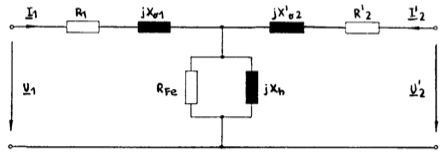
\includegraphics[width=6cm]{./bilder/VollstaendigesErsatzschaltbild.png} \end{minipage} &
					\begin{minipage}{4.5cm}
                    	\tiny
                    		$R_1, R_2'$: Widerstand Spule\\ \\
                    		$jX_{\sigma 1}, jX_{\sigma 2}'$: Streufluss Spule\\ \\
                    		$R_{Fe}$: Eisenverlust\\ \\
                    		$jX_h$: Hauptfluss Spule\\
                    \end{minipage} \\ \\
				Systemgleichung des realen Trafo &
					$\underline{U}_1 = R_1\cdot\underline{I}_1 + jX_{\sigma 1}\cdot\underline{I}_1 + jX_h\cdot(\underline{I}_1+\underline{I}_2')$ \\
					& $\underline{U}_2' = R_2'\cdot\underline{I}_2' + jX_{\sigma 2}'\cdot\underline{I}_2' + jX_h\cdot(\underline{I}_1+\underline{I}_2')$

            \end{tabular}
            	Für mittlere Transformatorenleistungen erbgeben sich etwa folgende Relationen zwischen
            	den einzelnen $R$s und $X$s:
            	$$ R_1 : R_2' : X_{\sigma 1} : X_{\sigma 2}' : X_h : R_{Fe} \approx 1:1:2:2:1000:10000	$$
            	
		\subsubsection{Leerlauf und Magnetisierung}
			\begin{tabular}{p{5cm}p{6cm}p{7cm}}
            	Rechnen &
            		\begin{minipage}{13cm}
                    	Mit Leerlaufdaten $R_{Fe}$ und $X_h$ ausrechnen. $R_1$ und $X_{\sigma1}$ vernachlässigen.
                    \end{minipage} \\ \\
            	Induktiver Leerlaufstrom &
            		\fbox{$\underline{I}_{10} = \underline{I}_{1Fe} + \underline{I}_{1\mu}$} $(\underline{I}_{1\mu} \gg \underline{I}_{1Fe})$ &
            		\begin{minipage}{8cm}
	            		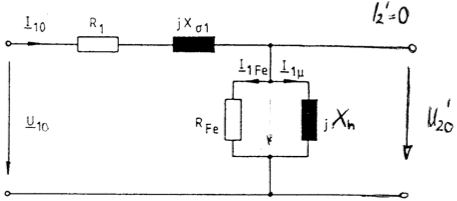
\includegraphics[width=5cm]{./bilder/ErsatzschaltbildTrafoLeerlauf.png}
	            	\end{minipage} \\ \\
				Magnetisierungsstrom &
					\fbox{$i_\mu = \sqrt{2}I_{\mu1}\cdot \sin(\omega t) + \sqrt{2}I_{\mu3}\cdot \sin(3\omega t) + \sqrt{2}I_{\mu m}\cdot \sin(m\omega t)$} &
					\hspace{3.3cm}$(m=2n+1 \hspace{0.3cm} n\epsilon \mathbb{N}_0)$ \\
					&
					Für den Effektivwert des Stromes: &
					\fbox{$I_{\mu RMS} = \sqrt{I_{\mu1}^2 + I_{\mu3}^2 +\ldots+ I_{\mu m}} $}\\ \\
				Leerlaufverluste &
					\fbox{$P_0 = P_{0Cu} + P_{0Hy} + P_{0Wi}$} \\
				Hystreseverluste &
					\fbox{$P_{Hy} \sim f \cdot B^2$} \\
				Wirbelstromverluste &
					\fbox{$v_W = c_W \cdot f^2 \cdot B^2$} &
					$c_W$ ist materialabhängige Konstante \\
				Relativer Leerlaufstrom &
					\fbox{$i_{0N} = \frac{I_{0N}}{I_{1N}}$} &
					$I_{1N}$ ist eingangsseitiger Nennstrom \\
				Eisenverluststrom &
					\fbox{$I_{Fe} = \frac{P_{0N}}{U_{1N}} = I_0 \cdot \cos(\varphi_0)$} \\
				Eisenverlustwiderstand &
					\fbox{$R_{Fe} = \frac{U_{1N}^2}{P_{0N}} = \frac{P_{0N}}{I_{Fe}^2}$} \\
				Hauptreaktanz &
					\fbox{$X_h = L_h \omega = \frac{U_{1N}}{I_{\mu}} = \frac{U_{1N}^2}{Q_{0N}}
					=
					\frac{Q_{0N}}{I_{\mu}^2}$} 
					& \fbox{$Q_{0N} = \sqrt{S_{0N}^2 - P_{0N}^2}$} \\
				Magnetisierungsstrom &
					\fbox{$I_\mu = I_{0N} \cdot \sin(\varphi_0) = \sqrt{I_0^2 - I_{Fe}^2}$} &
					\begin{minipage}{7cm}
                    	\begin{tabular}{p{2.5cm}p{3.5cm}}
	                    	\begin{minipage}{2.5cm}
	                        	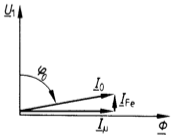
\includegraphics[height=1.5cm]{./bilder/ZeigerdiagrammRealerTrafoLeerlauf.png}
	                        \end{minipage} &
							\begin{minipage}{3.5cm}
	                       		oder \fbox{$\hat{I}_{\mu} = \frac{\hat{H}_{Fe} \cdot l_{Fe}}{N_1}$}
	                        \end{minipage}
						\end{tabular}
	            	\end{minipage} \\
				Leistungsfaktor im Leerlauf &
					\fbox{$\cos(\varphi_0) = \frac{P_{0N}}{I_{0N} \cdot U_{1N}}$} \\
            \end{tabular}
		\subsubsection{Kurzschluss}
			\begin{tabular}{p{6cm}p{6cm}p{6.5cm}}
            		\begin{minipage}{12cm}
                    	Mit Kurzschlussdaten $R_1$ und $X_{\sigma1}$ ausrechnen. $R_{Fe}$ und $X_h$ vernachlässigen.
                    \end{minipage} 
					& &	
					\multirow{3}{6.5cm}{
					%\begin{minipage}{7cm}
	            		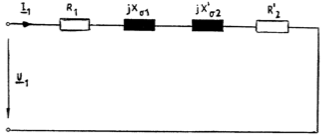
\includegraphics[height=2.5cm]{./bilder/KurzschlussErsatzschaltbild.png} } \\
	            	%\end{minipage}} \\
	            \\
				Kurzschlussimpedanz&
					\fbox{$\underline{Z}_k = R_k + jX_k$} \fbox{$Z_k = \frac{U_k}{I_k}$} \\
					& \fbox{$R_k = R_1 + R_2' = \cos{\varphi_k} \cdot Z_k  = \frac{P_k}{I_k^2}$}  \\
					& \fbox{$X_k = X_{\sigma1} + X_{\sigma2}' = \sin{\varphi_k} \cdot Z_k = \frac{Q_k}{I_k^2}$} \\
				Leistungsfaktor im Kurzschluss&
					\fbox{$\cos(\varphi_k) = \frac{P_k}{U_1 \cdot I_k} = \frac{P_k}{S_k}$} \\
             \end{tabular}

		\subsubsection{Spannungsänderung bei Belastung}
			\begin{tabular}{p{10cm}p{6cm}}
            		\begin{minipage}{10cm}
	            		\fbox{$\underline{U}_1 =
	            		\underline{U}_R+\underline{U}_X+\underline{U}_2'$} \qquad
	            		\fbox{$\underline{U}_2'=\underline{U}_2 \cdot "u$}\\ \\
	            		\fbox{$\underline{U}_R=R_k \cdot \underline{I}_1$} \qquad
	            		\fbox{$\underline{U}_X=jX_k \cdot \underline{I}_1$}\qquad
	            		\fbox{$\underline{I}_2' = \underline{I}_1$}\\
	            		\end{minipage} &
            		\begin{minipage}{6cm}
	            		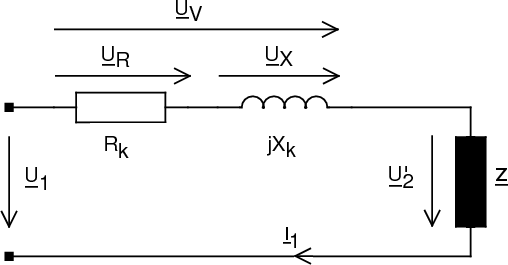
\includegraphics[width=5cm]{./bilder/ErsatzschaltbildTrafoLast.png}
	            	\end{minipage}\\			
            \end{tabular}\\ \\

			\begin{tabular}{p{8cm}|p{10cm}}
	 			\textbf{Zeigerdiagramme} & \textbf{Kappsches Dreieck}\\
				\begin{minipage}{8cm}
	            	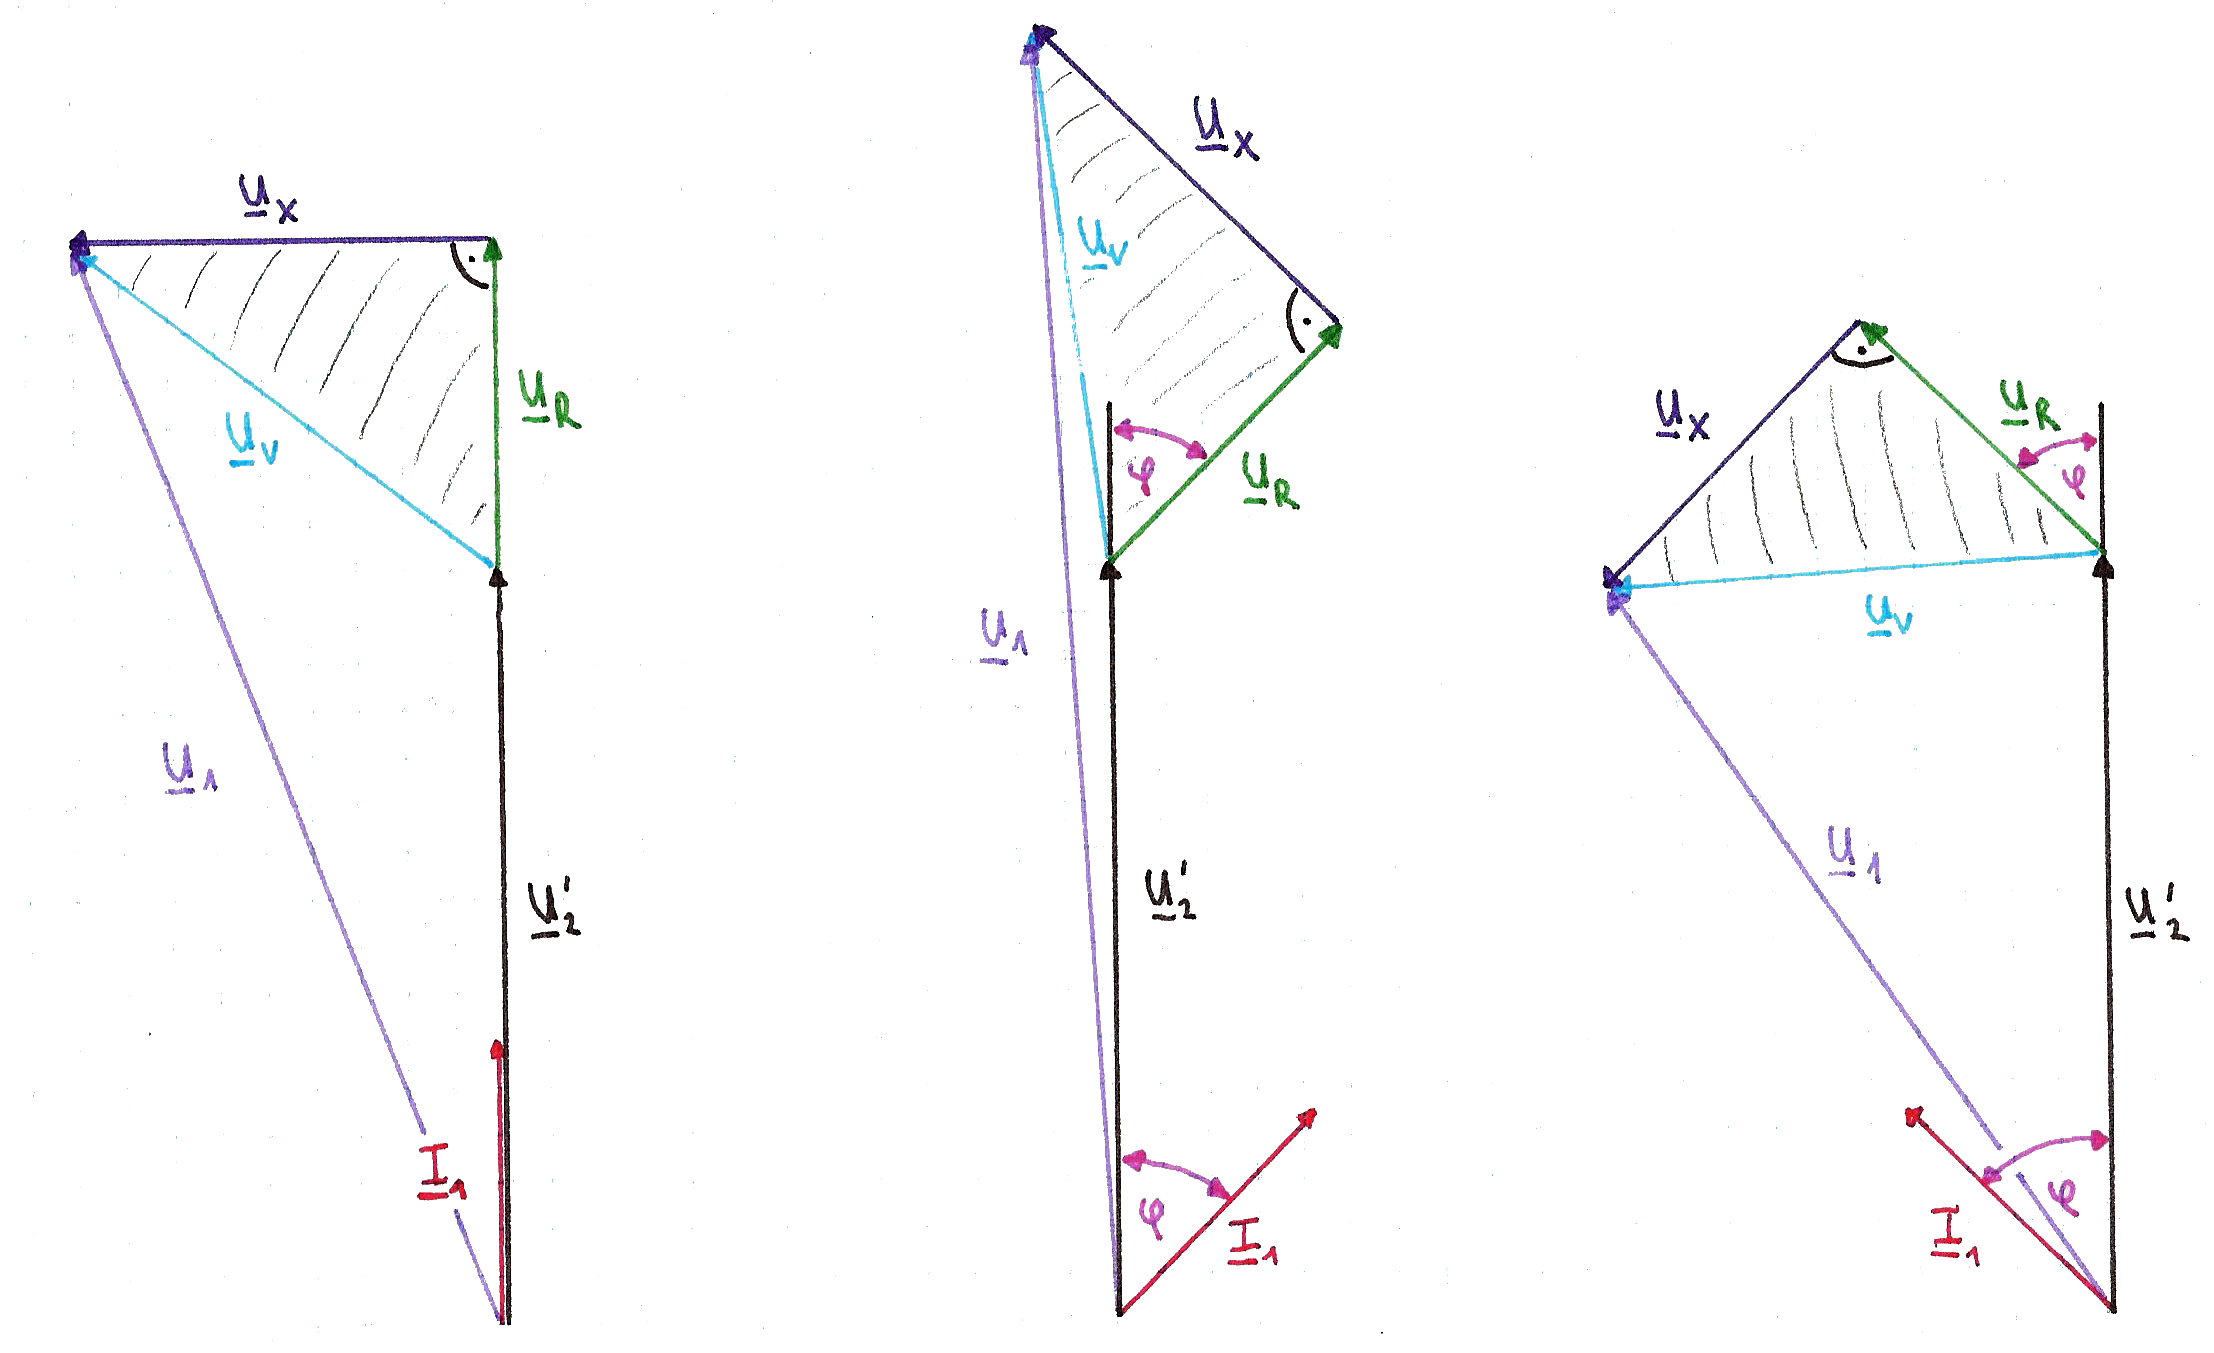
\includegraphics[width=8cm]{../WS_DST/bilder/KappschesDreieck_1.png}
	            \end{minipage}  & \hspace{0.2cm}
				\begin{minipage}{10cm} 
		        	\begin{minipage}{2.5cm}
						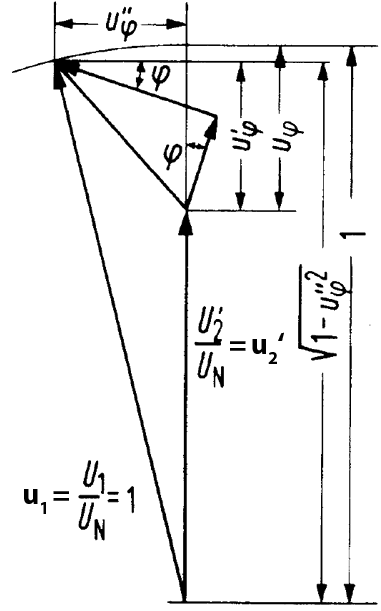
\includegraphics[width=3cm]{../WS_DST/bilder/KappschesDreieck.png}
		            \end{minipage}
					\begin{minipage}{7.5cm}
		      			$$u_{\varphi} = u_{\varphi'} + 1 - \sqrt{1 - u_{\varphi''}^2}$$
		      			$$ u_\varphi \approx u_{\varphi'}\quad (\text{für }u_k
		      			=\frac{U_k}{U_{N}} \cdot 100\% < 4 \%)$$
		      			$$u_{\varphi'} = u_r \cdot \cos \varphi + u_x
		      			\cdot \sin \varphi$$ $$u_{\varphi''} = u_x \cdot \cos \varphi - u_r \cdot \sin \varphi$$
		      			$$ u_r = \frac{R_k I}{U_N} \qquad u_x = \frac{X_k I}{U_N} $$
		      			$$ U_2 = \frac{U_N}{"u} - \Delta U_2 = \frac{U_1}{"u} - \frac{1}{"u}
		      			U_N u_\varphi $$\\
		      		\end{minipage}         
                \end{minipage}\\
				\begin{minipage}{8cm}
 					\begin{tabular}[c]{p{2.66cm}p{2.66cm}p{2.66cm}}
                     	$\quad \varphi = 0$ & $\quad\varphi > 0$ & $\quad\varphi
                     	< 0$\\ rein ohmsche & induktive & kapazitive\\
                     	Last & Last & Last\\
                     	&&\\
                     	&&\\
                     	&&\\
                     	&&\\
                     \end{tabular}               
                \end{minipage}& \hspace{0.2cm}
				\begin{minipage}{10cm}
		      		Beim kappschen Dreieck wird mit ``genormten'' Grössen (klein $u$) gerechnet: 
		      		$u = \frac{U_{Strang}}{U_{N, Strang}} = \frac{U_X}{U_1} \qquad
		      		\boldsymbol{U_N = U_1} $\\ \\ Das Kappsche Dreieck dreht sich um die
		      		Spitze der Primärspannung. Bei konstantem Strom und variablem $cos(\varphi)$ beschreibt ${u}_2'$
		      		einen
		      		Kreis um die Primärspannung.\\ Bei \textbf{kapazitiver Last steigt}
		      		die Sekundärspannung über den Leerlaufwert an. \\                  
                \end{minipage}     
            \end{tabular}

		
		\subsubsection{Wirkungsgrad des Trafos}
			\begin{tabular}{p{5cm}p{7cm}p{7cm}}
            	Wirkungsgrad &
            		\fbox{$\eta = 1-\dfrac{P_{V0} + P_{VK} \cdot
            		(\frac{P_B}{P_N})^2}{P_B} $} &
            	\begin{minipage}{7cm}
                	$P_B$ = Betriebsnennleistung\\
                	$P_{N}$ = Nennleistung\\
                	$P_{V0}$ = Leerlaufverlustleistung\\
                	$P_{VK}$ = Kurzschlussverlustleistung                	
                \end{minipage}\\ \\
            	 &
            		\fbox{$\eta = 1 - \dfrac{a + (\frac{P_B}{P_N})^2}{P_B} P_{VK}$} &
            	\begin{minipage}{7cm}
 					$a = \dfrac{P_{V0}}{P_{VK}}$                	
                \end{minipage}\\ \\            		
            	 &
            		\fbox{$\eta = 1 - \frac{P_{V0}+P_{VK}}{P_B} $} 
            		& (bei Wirkleistungsvollast) \\ \\
            	Maximaler Wirkungsgrad
            	& \fbox{$S_{\eta-max} = \sqrt{a} \cdot S_N$} \fbox{$P_{\eta-max} = \sqrt{a} \cdot
            	P_N$} 
            	& (Kupferverluste = Eisenverluste)
            \end{tabular}	

\newpage
	\subsection{Transformatoren Kühlmittel}
		\begin{center}
	    	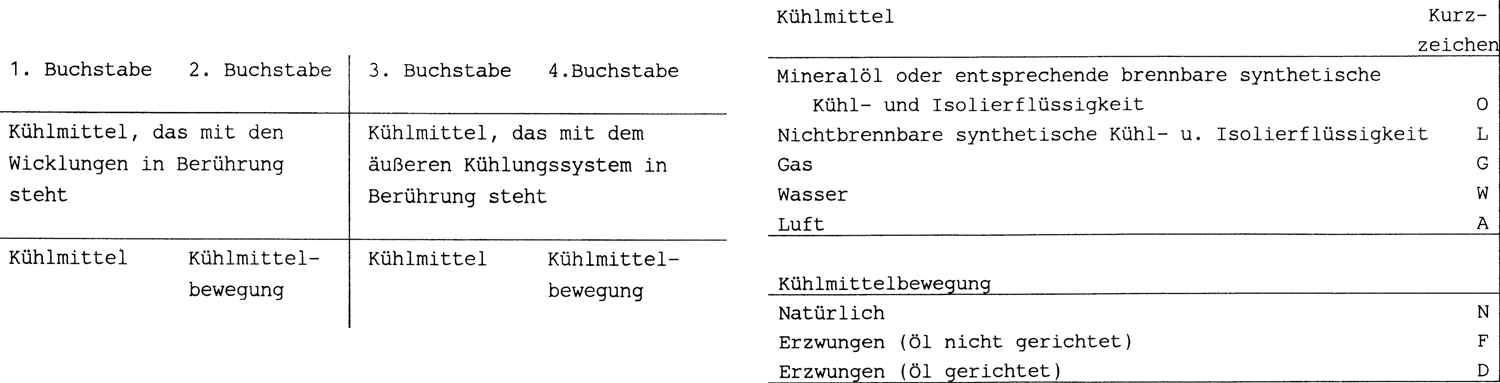
\includegraphics[width=19cm]{../WS_DST/bilder/Kuehlmittel.png}
	    \end{center} 

	\subsection{Drehstrom-Leistungstransformatoren} 
	Angegebene Leistung bezieht sich immer auf alle drei Wicklungen. $\Rightarrow P_{Wicklung} =
	\frac{P_N}{3}$ \\
	Angegebene Spannungen und Ströme gelten immer für Aussenleiter. Somit muss immer entweder - je
 nachdem ob Dreieck- oder Sternschaltung vorliegt -	Strom oder Spannung mit Faktor
 $\frac{1}{\sqrt{3}}$ multipliziert werden.
 	\subsubsection{Bauformen}
	 $$\text{Kennzeichnung} = [a][b][c][d] = \begin{cases}
                  [a] = \text{Oberspannungswicklung, Grossbuchstabe (Y,D,III,Z)
                  }\\
                  [b] = \text{Unterspannungswicklung, Kleinbuchstabe (y,d,iii,z) } \\
                  [c] \cdot 30^\circ = \text{Phasenverschiebung zwischen Unter- und Oberspannung }
                  \\ [d] = 0 \text{, falls Neutralleiter herausgeführt (optional)}
                  \end{cases}$$
		\begin{center}
	    	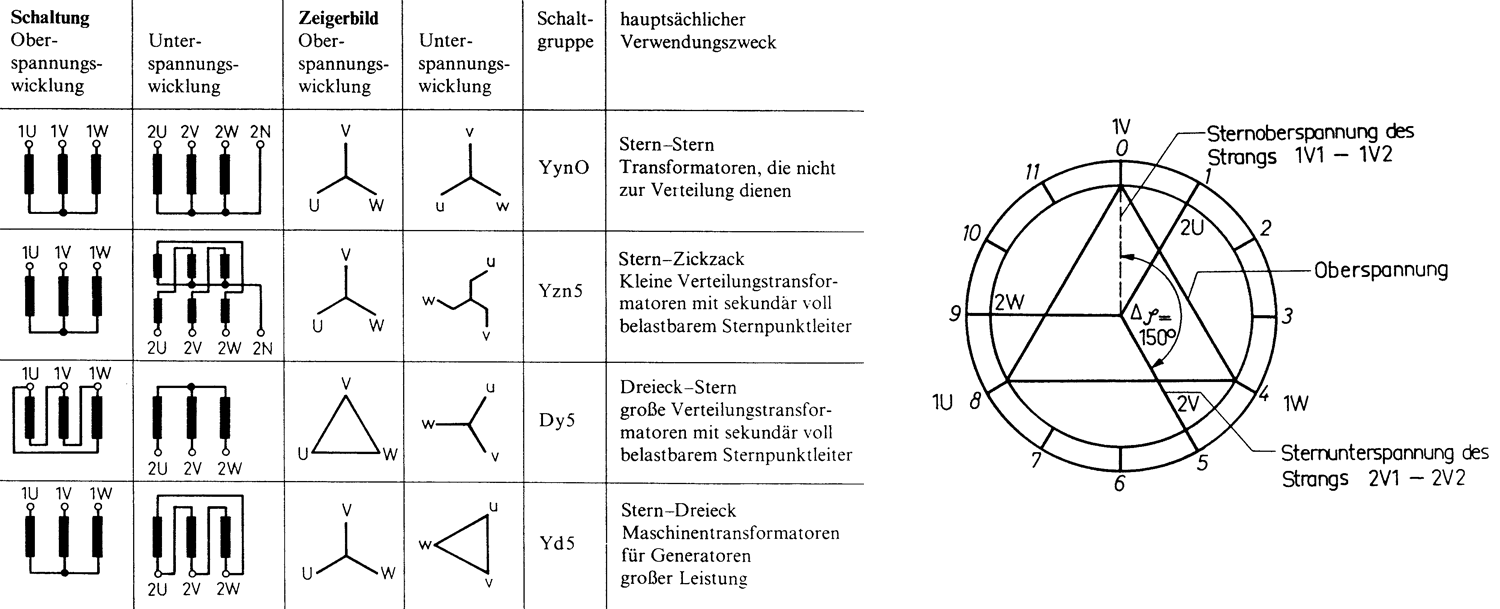
\includegraphics[height=6cm]{../WS_DST/bilder/Drehstromtrafo.png}
	    \end{center} 

\section{Dreiphasenwechselstrom (Drehstrom)}
	%\subsection{Entstehung des Drehstrom-Systems}
		\begin{tabular}{p{8.5cm}p{9cm}}
        	\begin{minipage}{8cm}
            	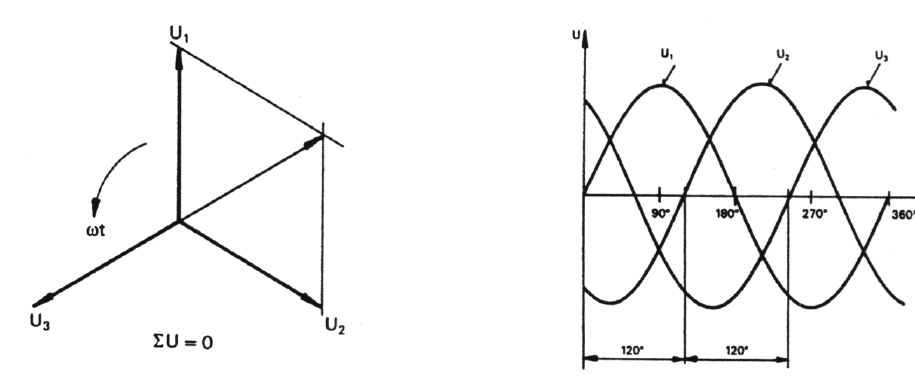
\includegraphics[width=7.5cm]{../WS_DST/bilder/Drehstrom.png}
            \end{minipage} &    
			\begin{minipage}{10cm}
            	Zeiger drehen mit $\omega t$ im Gegenuhrzeigersinn ($\omega > 0$). \\
            	$\underline{U}_2$ ist gegenüber $\underline{U}_1$ 
				$120^{\circ}$ nacheilend, $\underline{U}_3$ gegenüber $\underline{U}_1$ $240^{\circ}$.  \\ \\
				Somit gilt (bei symmetrischer Belastung): \\
				$\underline{U}_2 = \underline{U}_1 \cdot e^{j (-120^{\circ})}; \underline{U}_3
				= \underline{U}_1 \cdot e^{j (-240^{\circ})} = \underline{U}_1 \cdot e^{j
				(120^{\circ})}$
            \end{minipage}
        \end{tabular}
		
% 		\subsubsection{Verketten der Spannungen oder Ströme}
% 			\begin{tabular}{p{5cm}p{6cm}p{7cm}}
%             	\textbf{Maschensatz} &
%             		\fbox{$\underline{U}_1 + \underline{U}_2 + \underline{U}_3 = 0$} \\
%             	\textbf{Knotenpunktsatz} &
%             		\fbox{$\underline{I}_1 + \underline{I}_2 + \underline{I}_3 = 0$} \\
%             \end{tabular}

		\subsubsection{Stern- (Y) / Dreieckschaltung ($\Delta$)}
            	\renewcommand{\arraystretch}{1.5}
			\begin{tabular}{| p{4.5cm} | l | l |}
				\hline
	 				& Sternschaltung (Y)		& Dreieckschaltung ($\Delta$)\\
	 			\hline
	 			\vspace{0.2cm}
	 				%\textbf{Zeigerdiagramm} & & \\ 
	 				&
	 					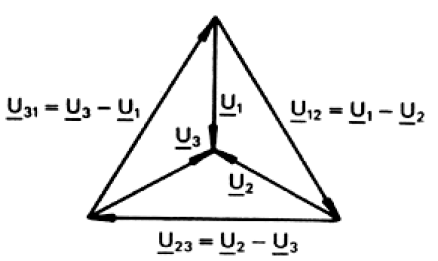
\includegraphics[width=5cm]{../WS_DST/bilder/Sternspannung.png} &
	 					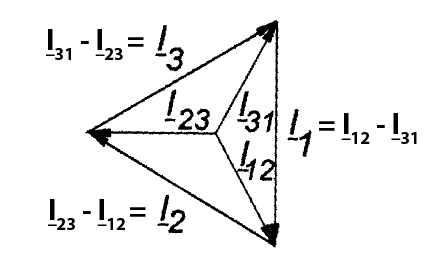
\includegraphics[width=5cm]{../WS_DST/bilder/Dreieckstrom.png} \\
	 				
		 			Verkettete Spannung &
		 				$U = U_{Str} \cdot \sqrt{3}$ \hspace{0.2cm} $\underline{U} = \underline{U}_{Str} \cdot \sqrt{3} \cdot e^{j 30^\circ}$ &
		 				$U = U_{Str}$ \hspace{0.2cm} $\underline{U} = \underline{U}_{Str}$ \\
		 			Aussenleiterströme &
		 				$I = I_{Str}$ \hspace{0.2cm} $\underline{I} = \underline{I}_{Str}$ &
		 				$I = I_{Str} \cdot \sqrt{3} $ \hspace{0.2cm} $\underline{I} =
		 				\underline{I}_{Str} \cdot \sqrt{3} \cdot e^{-j 30^\circ} $ \\ Gesamt-Scheinleistung &
		 				$S = 3 \cdot S_{Str} =\sqrt{3} \cdot U \cdot I $ \hspace{0.2cm} in $[VA]$
		 				& $S = 3 \cdot S_{Str} = \sqrt{3} \cdot U \cdot I$ \hspace{0.2cm} in $[VA]$ \\ Scheinleistung pro Strang &
		 				\multicolumn{2}{l|}{\hspace{3cm} $S_{Str} = U_{Str} \cdot I_{Str}$ \hspace{0.2cm} in $[VA]$} \\
		 			Wirkleistung &
		 				\multicolumn{2}{l|}{\hspace{3cm} $P = S \cdot \cos\varphi = \sqrt{3} \cdot U \cdot I \cdot \cos\varphi$ \hspace{0.2cm} in $[W]$} \\
		 			Blindleistung &
		 				\multicolumn{2}{l|}{\hspace{3cm} $Q = S \cdot \sin\varphi = \sqrt{3} \cdot U \cdot I \cdot \sin\varphi$ \hspace{0.2cm} in $[var]$} \\
% 		 			Wirkarbeit &
% 		 				\multicolumn{2}{l|}{\hspace{3cm} $W = P \cdot t = \sqrt{3} \cdot U \cdot I \cdot cos\varphi \cdot t$ \hspace{0.2cm} in $[Ws, kWh]$} \\
% 		 				&\multicolumn{2}{c|}{}\\
% 		 			Blindarbeit &
% 		 				\multicolumn{2}{l|}{\hspace{3cm} $W_b = Q \cdot t = \sqrt{3} \cdot U \cdot I \cdot sin\varphi \cdot t$ \hspace{0.2cm} in $[varh, kvarh]$} \\
	 			\hline
			\end{tabular}
        \renewcommand{\arraystretch}{1}
		
		%\subsubsection{Bestimmung des Y-Punktes mittels Leitwert-Operatoren im Vierleiter-Drehstromnetz}
        \subsubsection{Ausfall des Neutralleiters: Bestimmung des Y-Punktes mittels Leitwert-Operatoren}
            \begin{tabular}{p{5cm}p{13cm}}
            	\begin{minipage}{8cm}
                	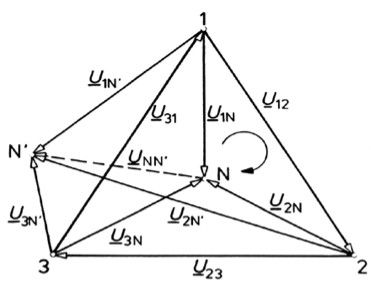
\includegraphics[width=5cm]{../WS_DST/bilder/ZeigerdarstellungVerschobenerSternpunkt.png}
                \end{minipage} &
				\begin{minipage}{13cm}
                	$\underline{U}_{12} = \underline{U}_{1N'} - \underline{U}_{2N'}$ \hspace{0.3cm}
                	$\underline{U}_{1N'} = \underline{U}_{1N} + \underline{U}_{NN'}$ \hspace{0.3cm}
                	$\underline{I}_1 = \underline{Y}_1 \cdot \underline{U}_{1N'} = \underline{Y}_1 \cdot (\underline{U}_{1N} + \underline{U}_{NN'})$ \\
                	$\underline{U}_{23} = \underline{U}_{2N'} - \underline{U}_{3N'}$ \hspace{0.3cm}
                	$\underline{U}_{2N'} = \underline{U}_{2N} + \underline{U}_{NN'}$ \hspace{0.3cm}
                	$\underline{I}_2 = \underline{Y}_2 \cdot \underline{U}_{2N'} = \underline{Y}_2
                	\cdot (\underline{U}_{2N} + \underline{U}_{NN'})$ \\ $\underline{U}_{31} = \underline{U}_{3N'} - \underline{U}_{1N'}$ \hspace{0.3cm}
                	$\underline{U}_{3N'} = \underline{U}_{3N} + \underline{U}_{NN'}$ \hspace{0.3cm}
                	$\underline{I}_3 = \underline{Y}_3 \cdot \underline{U}_{3N'} = \underline{Y}_3
                	\cdot (\underline{U}_{3N} + \underline{U}_{NN'})$ \\ \\ 
                	$$\underline{U}_{NN'} = \boldsymbol{-} \frac{(\underline{Y}_1 \cdot
                	\underline{U}_{1N} + \underline{Y}_2 \cdot \underline{U}_{2N} + \underline{Y}_3 \cdot
                	\underline{U}_{3N})}{\underline{Y}_1 + \underline{Y}_2 +
                	\underline{Y}_3}$$
                \end{minipage}
			\end{tabular}

%		\subsubsection{Anwendung der Y- und $\Delta$- Schaltung}
	
	\subsection{Stern-Dreieck-Umwandlung}% \formelbuch{18}}
	%\begin{figure}
	  \begin{minipage}[lt]{7.5 cm}
	    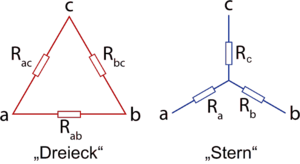
\includegraphics[width=6cm]{./bilder/stern-dreieck.png} 
	  \end{minipage}
	  \begin{minipage}[rt]{9.35 cm} %BASTEL!!
      \renewcommand{\arraystretch}{2}
	  \begin{tabular}{ll}
	Umwandlung $\triangle \rightarrow Y$: 
		&$Z_{c} = \dfrac{Z_{ac} Z_{bc}}{Z_{ab}+Z_{bc}+Z_{ac}}$\\
	Umwandlung $Y \rightarrow \triangle$: 
		&$Y_{ac}=\dfrac{Y_{a} Y_{c}}{Y_{a}+Y_{b}+Y_{c}}$\\
	Bei gleichen Widerständen:
	&$R_Y = \frac{R_\triangle}{3}$ \\
	Bei gleichen Kapazitäten:
	&$C_Y = C_\triangle \cdot 3 $ \\
	Bei gleichen Induktivitäten:
	&$L_Y = \frac{L_\triangle}{3}$
	  \end{tabular}
      \renewcommand{\arraystretch}{1}
	  \end{minipage}
	%\end{figure}
	
	\subsection{Defektleistung von symmetrischen Drehstromverbrauchern}
		\begin{tabular}{| p{7.5cm} | l | l |}
			\hline
 				& Normalleistung		& Defektleistung\\
 			\hline
	 			\textbf{Y-Schaltung bei Leiter- oder Strangausfall} ohne Neutralleiter &
	 				$P_{Norm} = 3 \cdot \frac{U^2_{Str}}{R} = \frac{U^2}{R}$ &
	 				$P_{Def} = \frac{1}{2} \frac{U^2}{R}$ \tiny{nur 50\% von $P_{Norm}$} \\
	 			&&\\
	 			\textbf{Y-Schaltung bei Leiter- oder Strangausfall} mit Neutralleiter &
	 				$P_{Norm} = 3 \cdot \frac{U^2_{Str}}{R} = \frac{U^2}{R}$ &
	 				$P_{Def} = 2 \cdot \frac{U^2_{Str}}{R} = \frac{2}{3} \frac{U^2}{R}$ \tiny{nur 66\% von
	 				$P_{Norm}$} \\ &&\\
	 			\textbf{$\Delta$-Schaltung bei Leiterausfall} &
	 				$P_{Norm} = 3 \cdot \frac{U^2}{R}$ &
	 				$P_{Def} = \frac{U^2}{R} + \frac{U^2}{2R} = \frac{3U^2}{2R}$ \tiny{nur 50\% von $P_{Norm}$} \\
	 			&&\\
	 			\textbf{$\Delta$-Schaltung bei Strangausfall} &
	 				$P_{Norm} = 3 \cdot \frac{U^2}{R}$ &
	 				$P_{Def} = 2 \cdot \frac{U^2}{R}$ \tiny{nur 66\% von $P_{Norm}$} \\
	 		\hline
		 \end{tabular} 

% 	\subsection{Messen der Drehstromleistung}
% 	\subsection{Kompensation im Drehstromnetz}
%%%%%%%%%%%%%%%%%%%%%%%%%%%%%%%%%%%%%%%%%%%%%%%%%%%%%%%%%%%%%%%%%%%%%%%%%%%%%%%%%%%%%%%%%%%%%%%%	
% \section{Komplexe Zahlen mit Taschenrecher - Texas Instruments}
% 	\begin{tabular}{p{4cm}p{10cm}}
% 	$\ldots \triangleright Rect $ 		& Umwandlung in Kartesische Darstellung \\
% 	$\ldots \triangleright Polar $ 		& Umwandlung in Polare Darstellung \\
% 	$conj(\ldots)$ 						& Konjugiert Komplex $\overline{z}$\\
% 	$abs(\ldots) $						& Betrag $|z|$\\
% 	$angle(\ldots) $					& Winkel $arg(z)$\\
% 	$imag(\ldots) $	s					& Imaginärteil $Im(z)$ \\
% 	$real(\ldots) $						& Realteil $Re(z)$ \\
% 	\end{tabular}

%%%%%%%%%%%%%%%%%%%%%%%%%%%%%%%%%%%%%%%%%%%%%%%%%%%%%%%%%%%%%%%%%%%%%%%%%%%%%%%%%%%%%%%%%%%%%%%%
%%%%%%%%%%%%%%%%%%%%%%%%%%%%%%%%%%%%%%%%%%%%%%%%%%%%%%%%%%%%%%%%%%%%%%%%%%%%%%%%%%%%%%%%%%%%%%%%


\end{document}